\documentclass{article}
\usepackage{tikz}

\begin{document}
	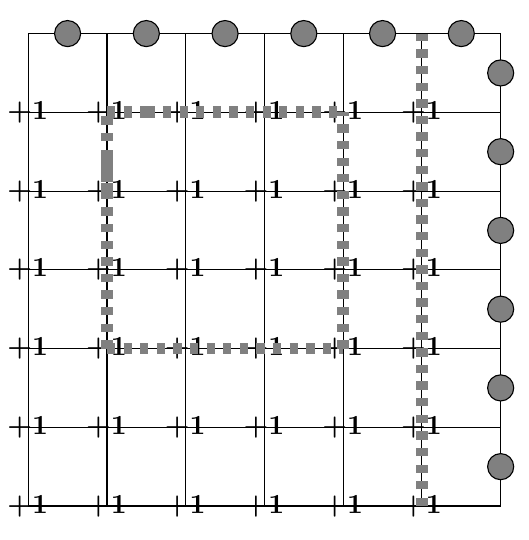
\begin{tikzpicture}
		
		
		% Draw solid grid and nodes with circles in the middle of each side
		\draw[step=1cm] (-3,-3) grid (3,3);
		\foreach \i in {-2.5,...,2.5}
		{
			\foreach \j in {-2.5,...,2.5}
			{
				
				
				\begin{scope}[transform canvas={xshift=\i cm,yshift=\j cm}]
					\node[right,xshift=0.2cm,yshift=0.4cm] {};
					% Convert \j and \i to integers
					\pgfmathtruncatemacro{\intj}{\j}
					\pgfmathtruncatemacro{\inti}{\i}
					
					% Draw circles at the midpoints of each side
					\ifnum\intj=2
					\draw node[draw,circle,fill=gray] at (0,0.5) {};
					\fi
					
					\ifnum\inti=2
					\draw node[draw,circle,fill=gray] at (0.5,0) {};
					\fi
					
					\draw node[label=left:\textbf{+1}] at (0,-0.5) {};
				
				\end{scope}
			}
		}
		
		\foreach \i in {-2,...,-2}
		{
			\draw[dashed,black!50, line width=1.5mm] (\i,-1) -- (\i,1.5);
			
			
			\draw[dashed,black!50, line width=1.5mm] (\i,1) -- (\i,2);
		
		
			
		}
		
		\foreach \j in {2,...,2}
		{
			
			\draw[dashed,black!50, line width=1.5mm] (-2, \j) -- (-1.5, \j);
			
			
			\draw[dashed,black!50, line width=1.5mm] (-1.5, \j) -- (1, \j);
		
			
		}
		
		
		\foreach \i in {1,...,1}
		{
			\draw[dashed,black!50, line width=1.5mm] (\i,-1) -- (\i,2);
		
			
		}
		
		\foreach \j in {-1,...,-1}
		{
			\draw[dashed, black!50, line width=1.5mm] (-2, \j) -- (1, \j);
		
		
		}
		
		
		\foreach \i in {2,...,2}
		{
			\draw[dashed,black!50, line width=1.5mm] (\i,-3) -- (\i,3);
		
			
		}
		
		
	\end{tikzpicture}
\end{document}
